\section{Hardware}
\label{sec:Hardware}
 
 To ensure a right positioning of the fibres in the fibre mat a setup consisting of an industrial camera and a lens with a big magnification is used. A scheme of the setup can found in Fig. \ref{hardwarescheme}. Die Camera system is mounted on the same slide as the positioning spool. As a result the camera is moving along the width of the wheel and monitors always the current fibre. Furthermore the camera will have a tangential look an the wheel. A schematic picture of the camera is shown in Fig. \ref{viewscheme}. The fibres of the first layer are guided by the threat in the wheel and are well positioned. The dark blue fibre is the current one and should be monitored very precisely. 
\begin{figure}[tb]
\begin{center}
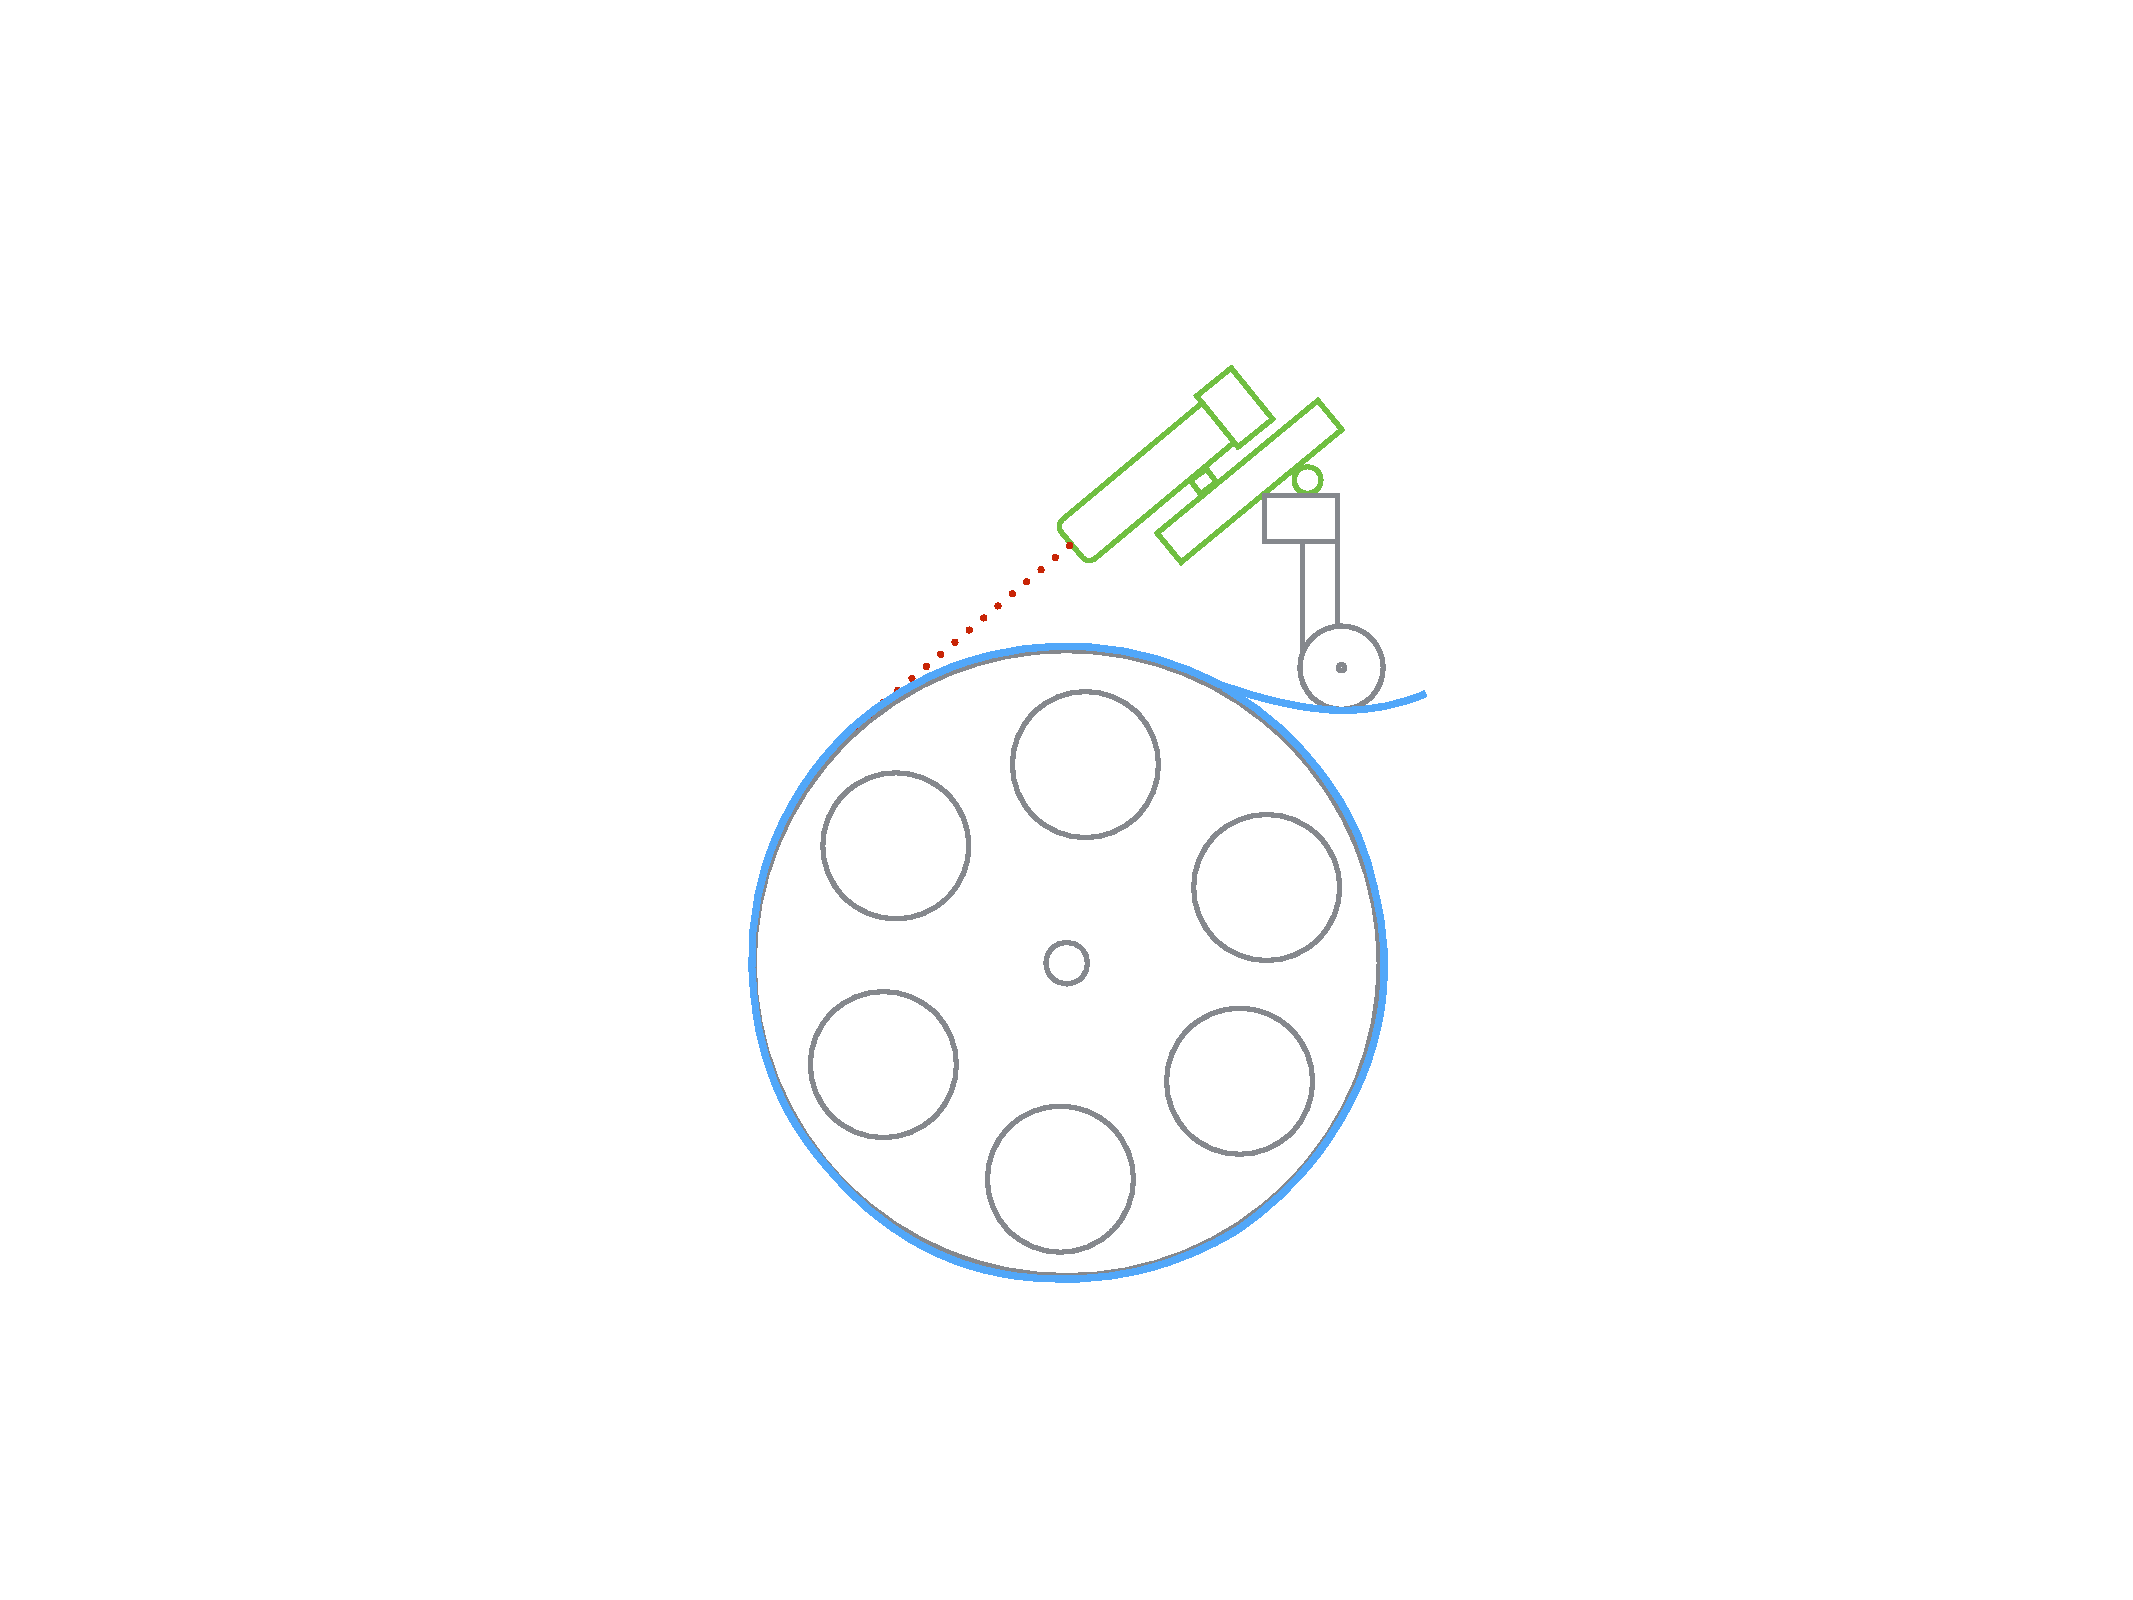
\includegraphics[width=0.5\linewidth]{figs/hardwarescheme.pdf}%
\caption{Scheme of the camera setup on the winding maschine. The camera (green) will be placed on the same slide as the positioning spool and look tangential on the wheel. \label{hardwarescheme}}
\end{center}
\end{figure}
\begin{figure}[tb]
\begin{center}
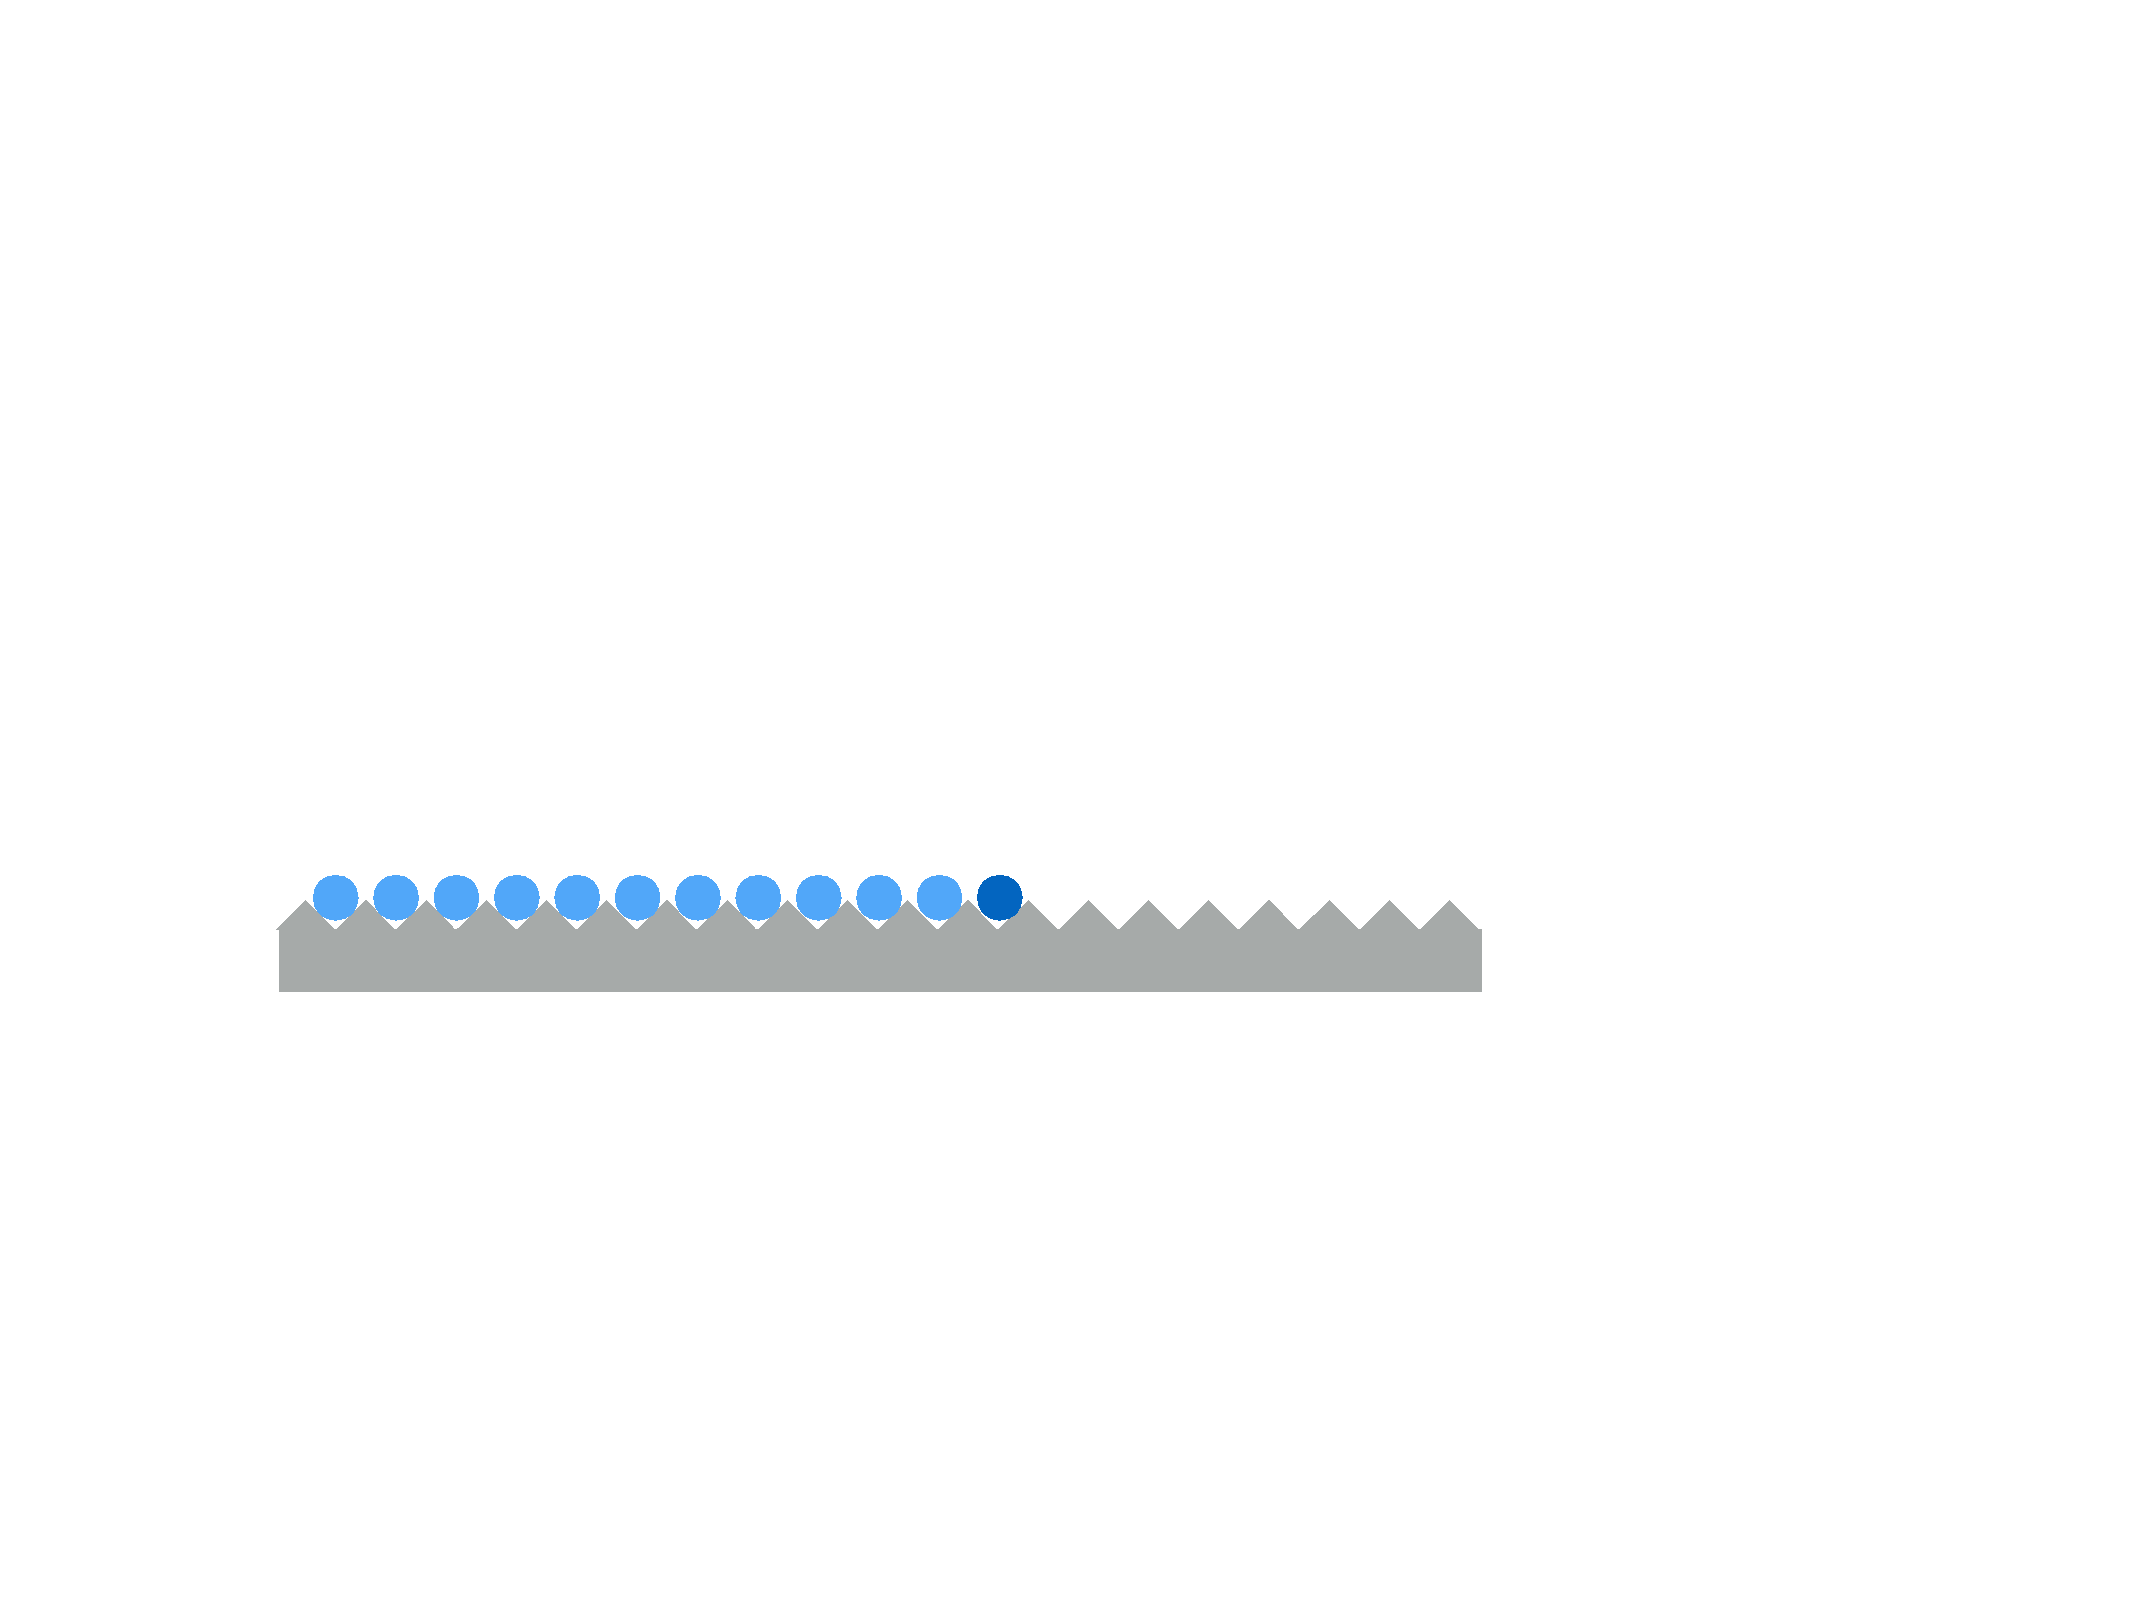
\includegraphics[width=0.5\linewidth]{figs/viewscheme.pdf}%
\caption{Scheme of the view if the camera looks tangential on the wheel. Fibres in the first layer are guided by the threat in the wheel. The current fibre is marked in dark blue.\label{viewscheme}}
\end{center}
\end{figure}

Despite of the many influences which have a bearing on the fibre positioning, there are only two different effects which can be observed during the winding process. On the one hand a fibre can jump in the wrong threat an leave an empty space (see Fig. \ref{fig:errors1})).On the other hand a fibre is able to lie down in the next layer (see Fig. \ref{fig:errors2}).
\begin{figure}[ht]
\centering
\subfigure[]{
   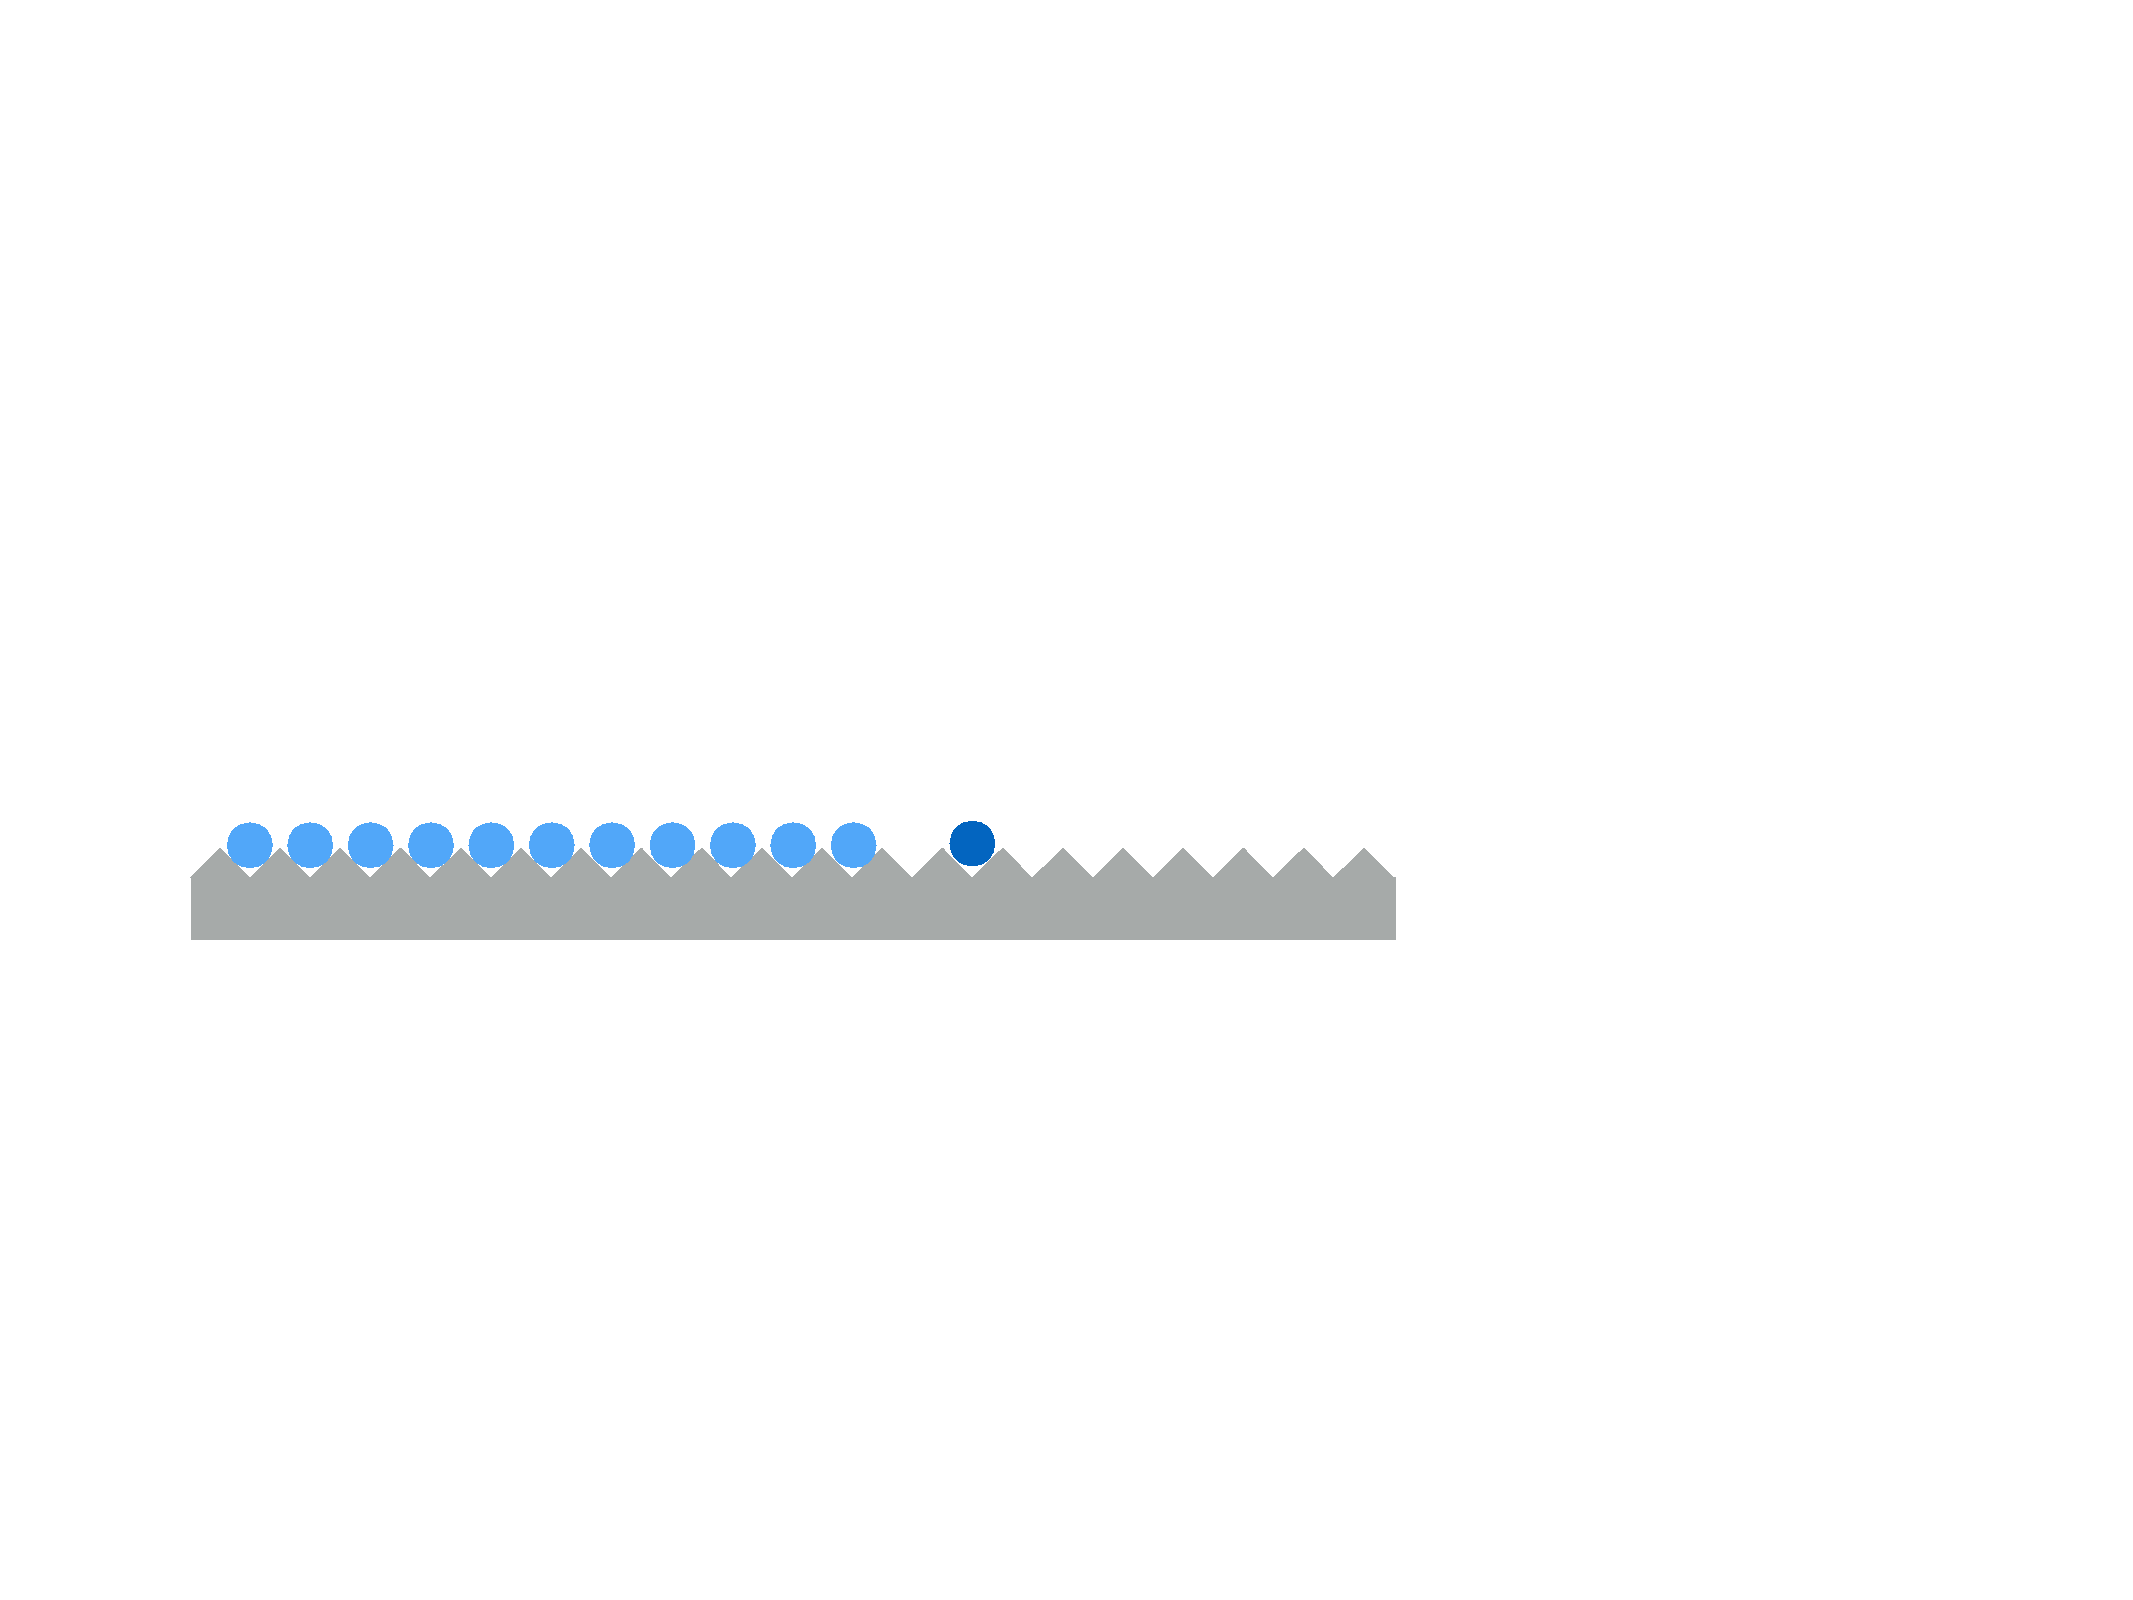
\includegraphics[width=0.4\textwidth] {figs/viewempty.pdf}
   \label{fig:errors1}
 }
\quad
 \subfigure[]{
   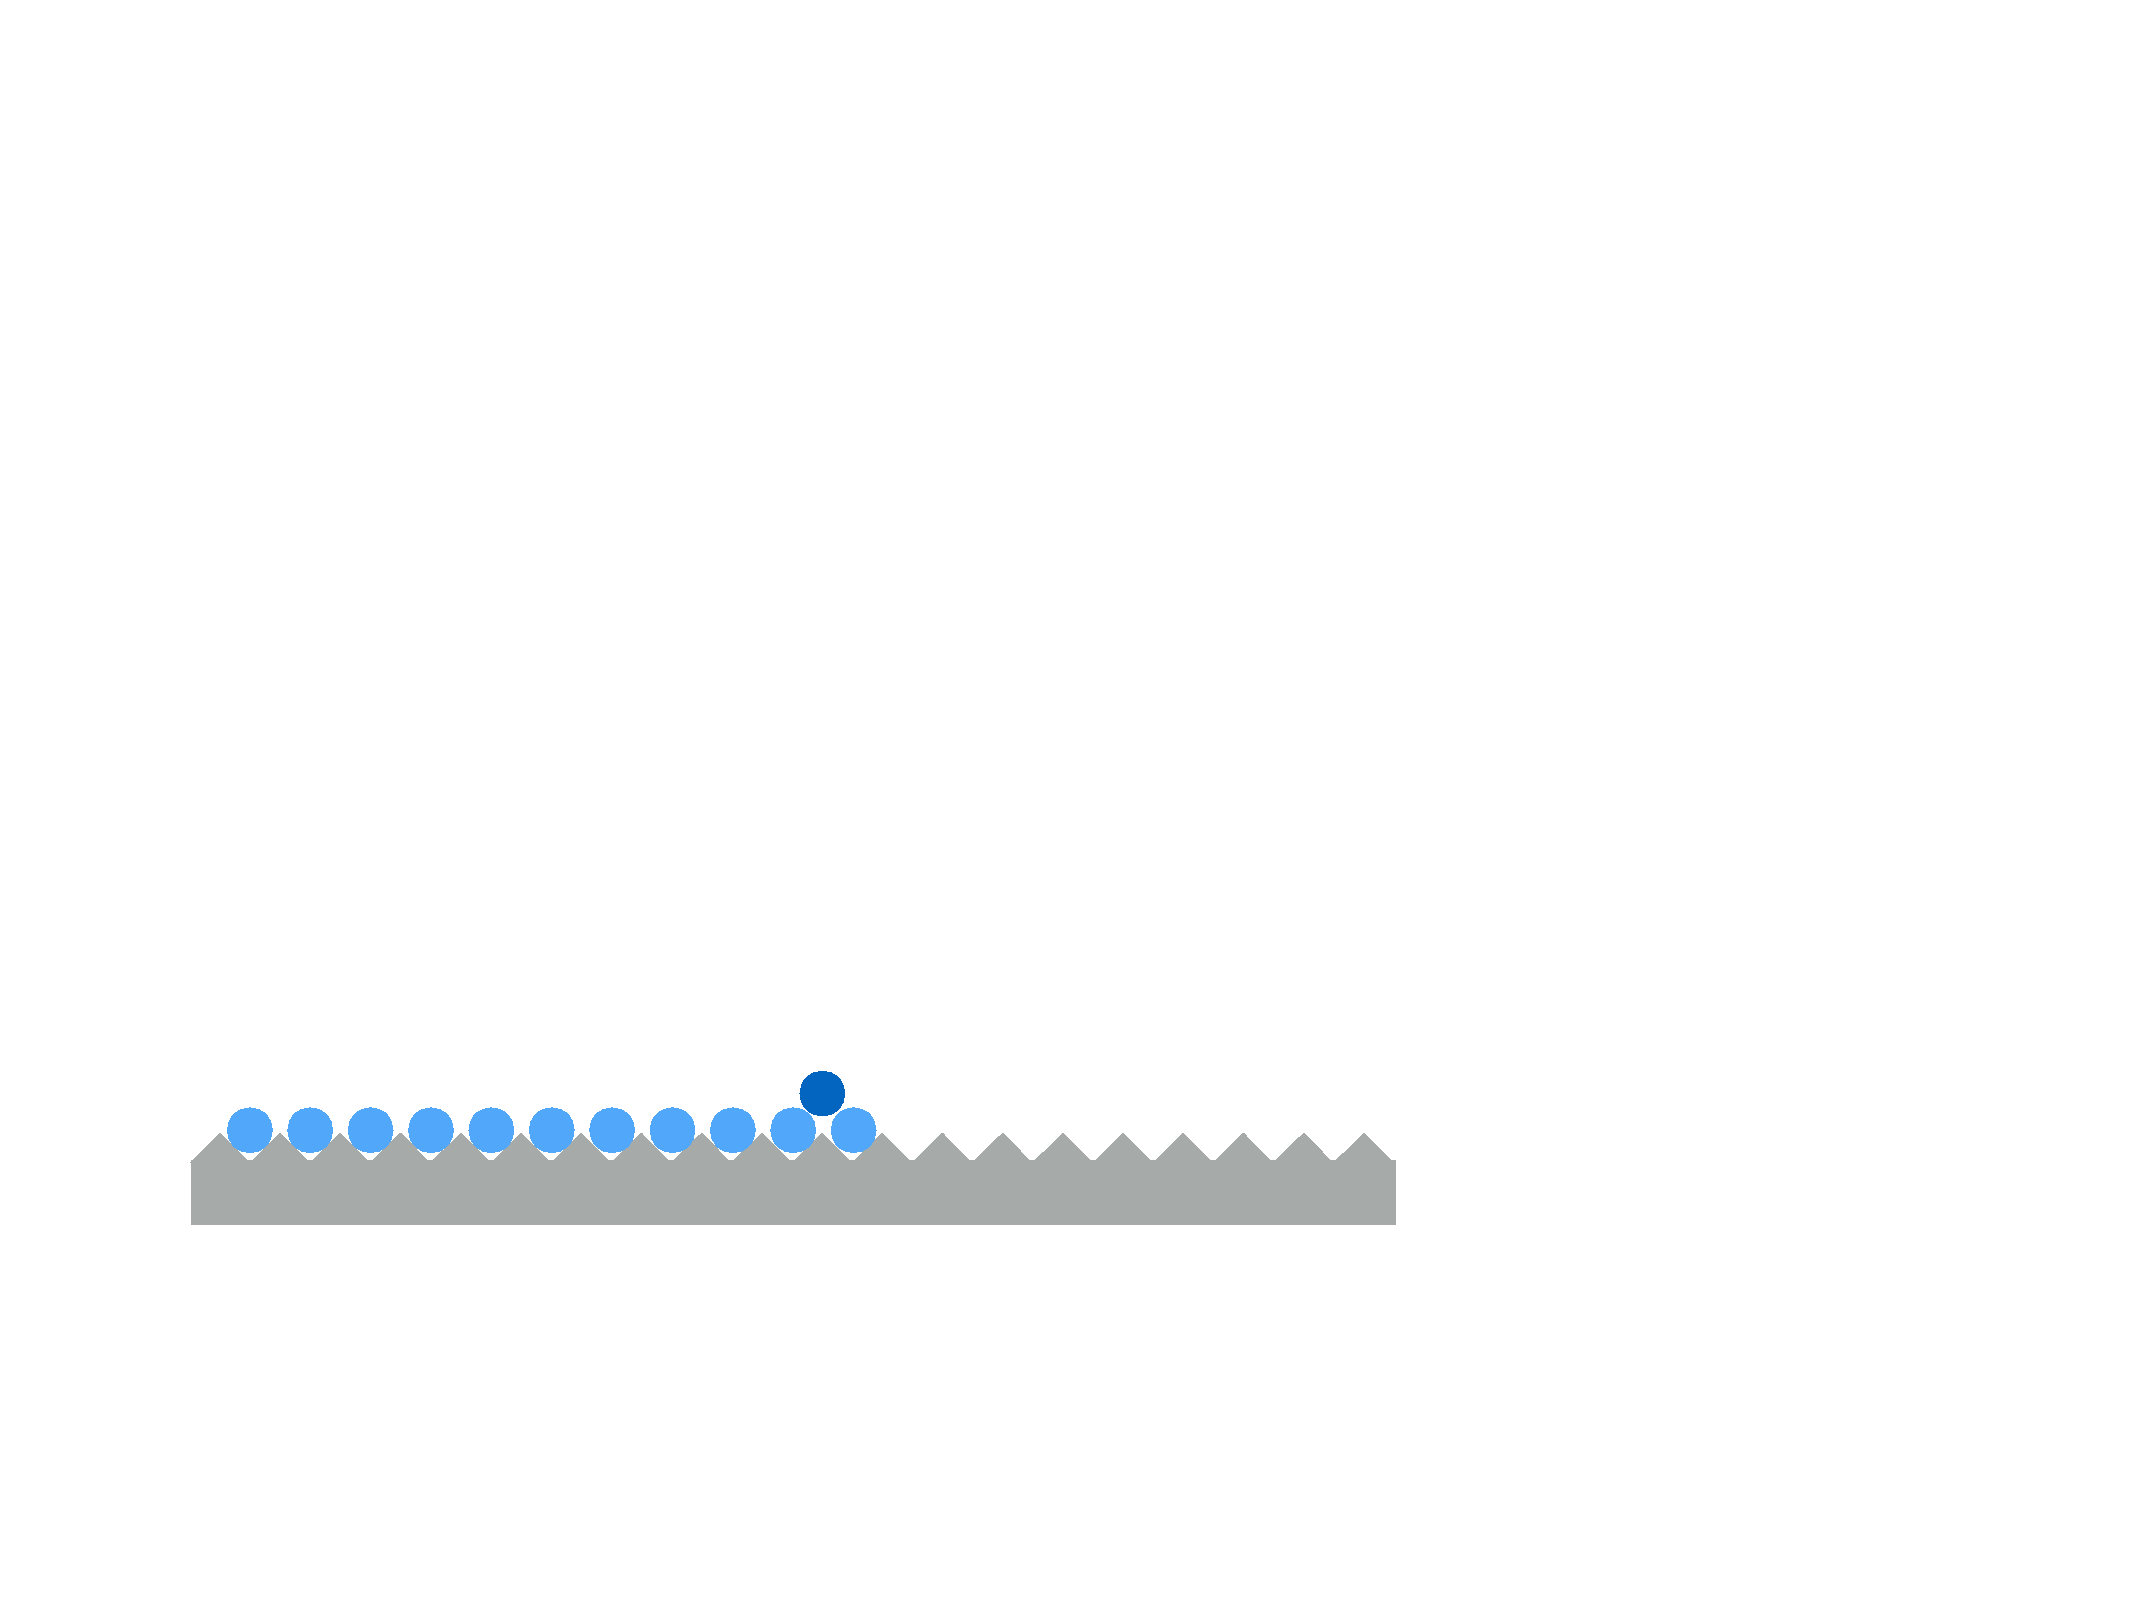
\includegraphics[width=0.4\textwidth] {figs/viewjump.pdf}
   \label{fig:errors2}
 }
\label{errors}
\caption{Two different defects which can occur during the winding process. In (a) the current fibre jumped in the wrong threat and leave an empty space. (b) shows a fibre lying in the wrong layer.}
\end{figure}

A picture of the current hardware setup is shown in Fig. \ref{CameraOnMaschine}. The camera can be adjusted by a ball head. Unfortunately the lens has no possibilty to adjust the focus, so that another slide is used for this.
\begin{figure}[tb]
\begin{center}
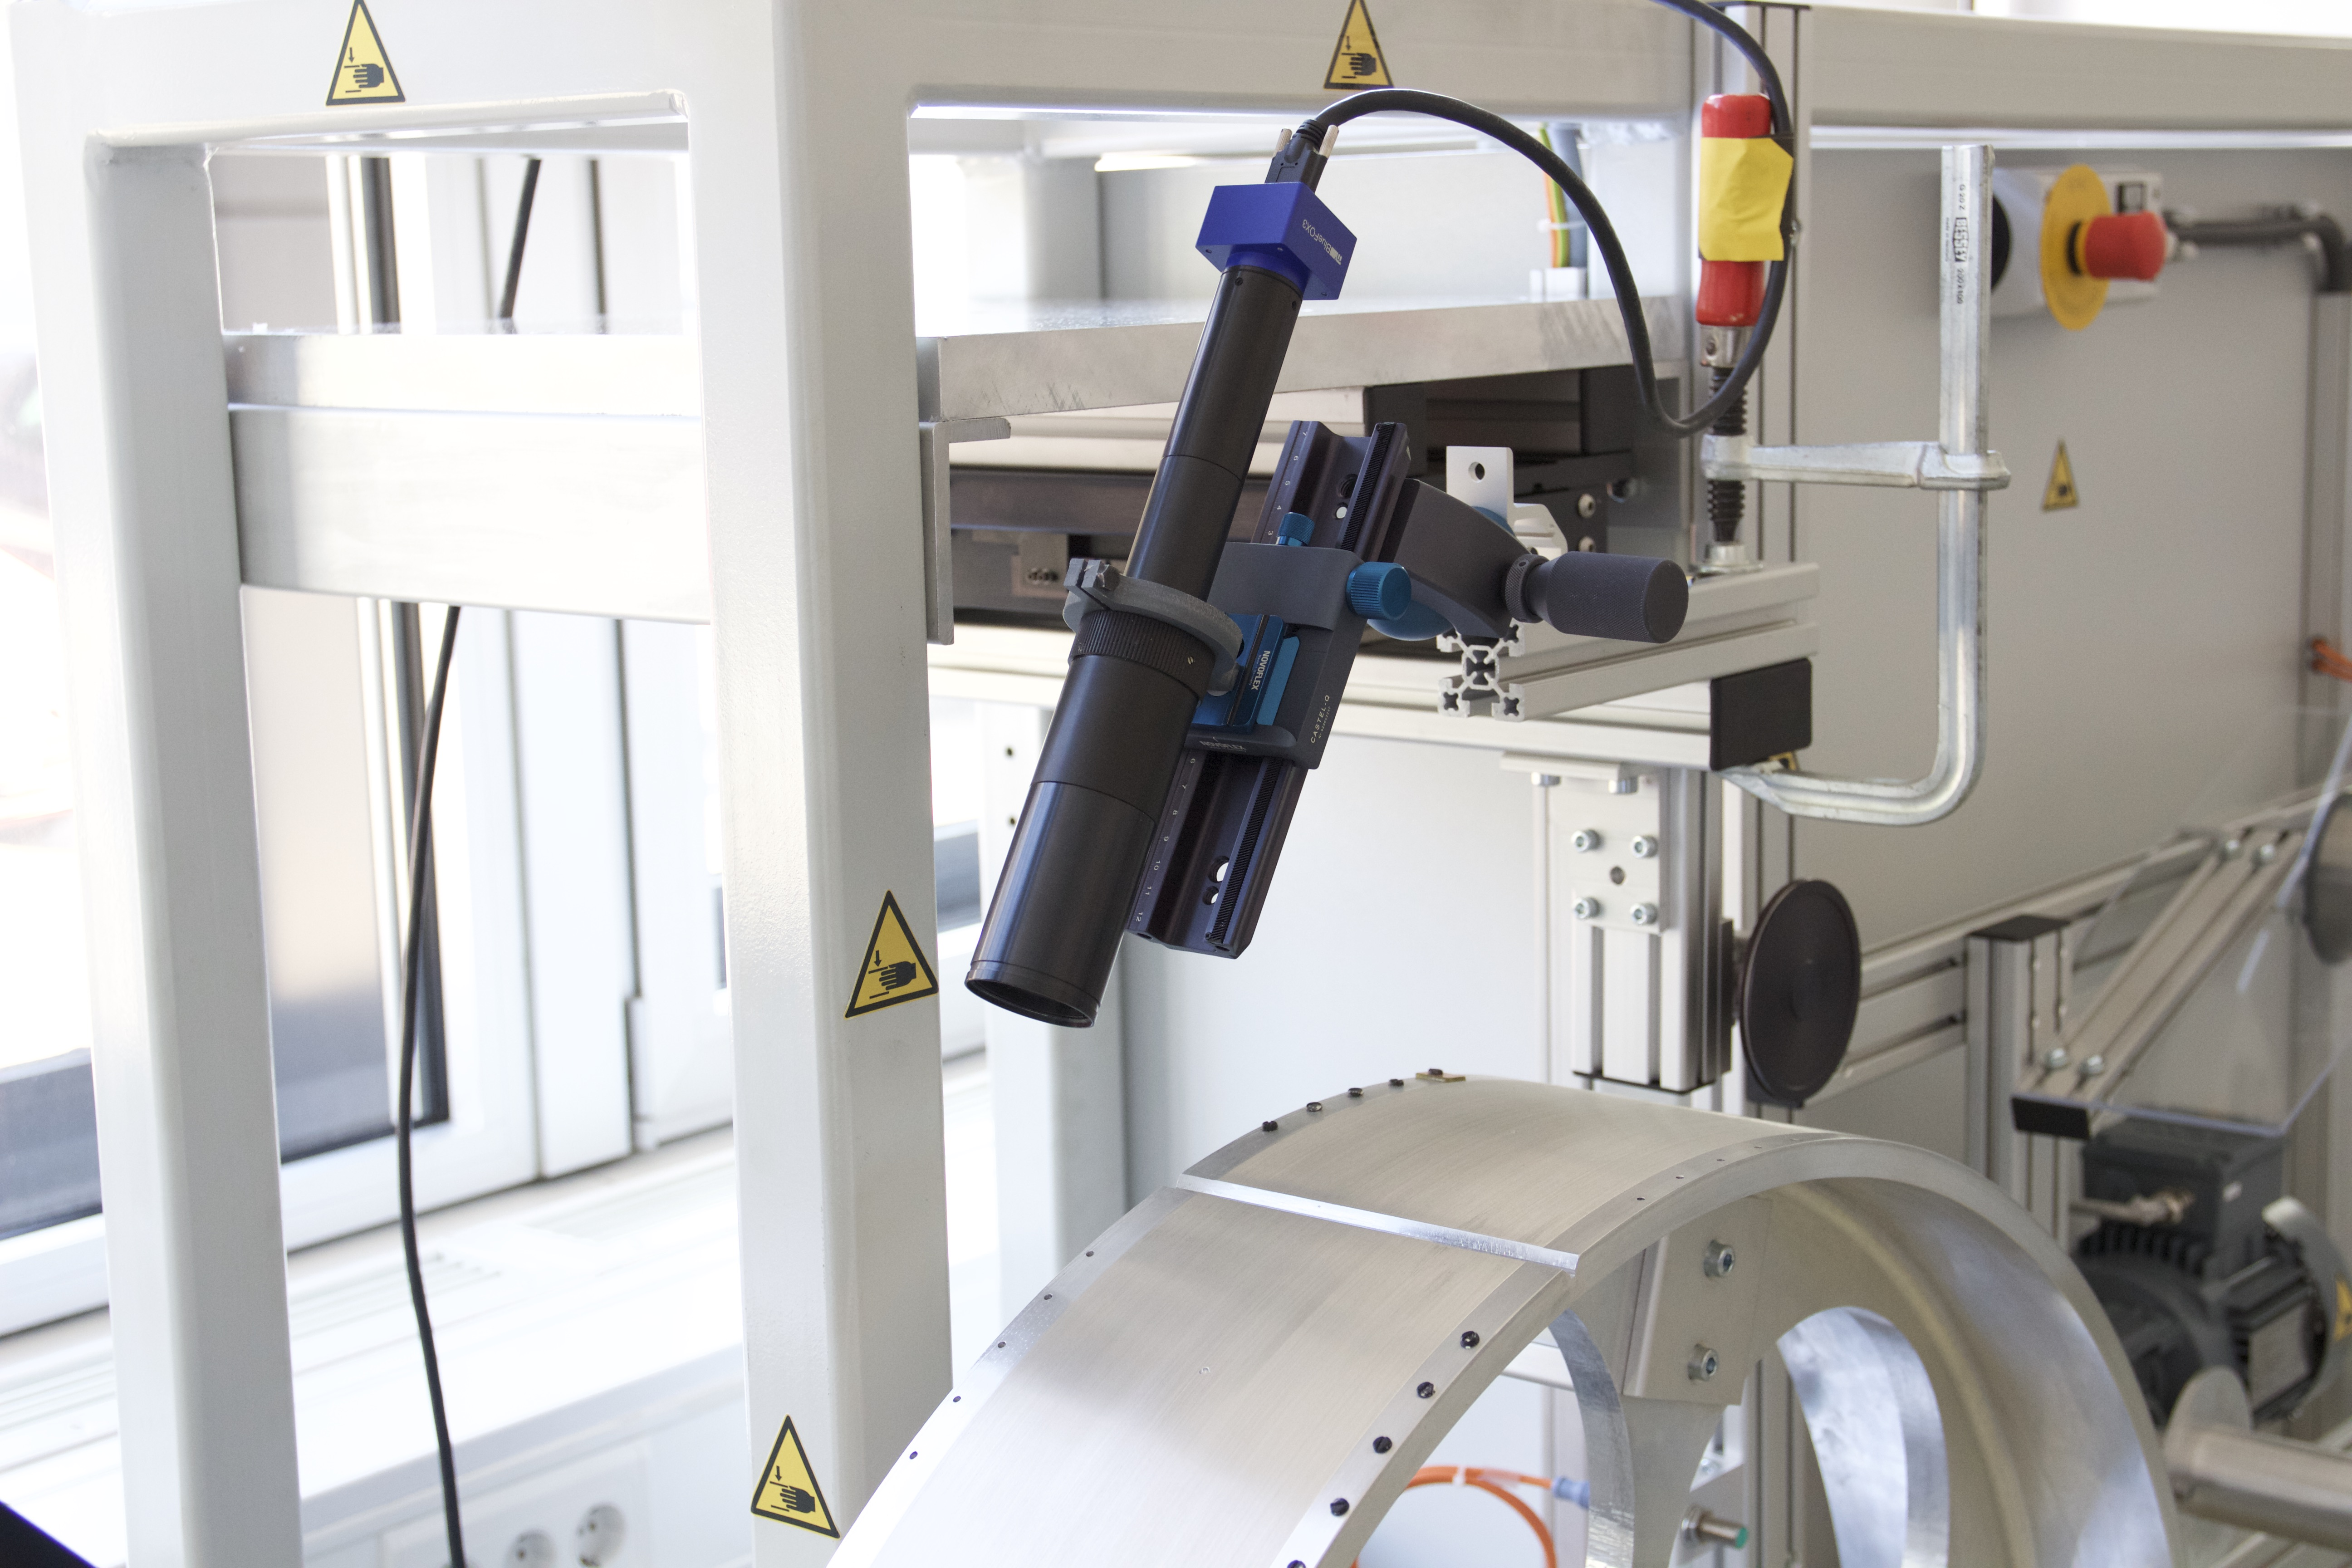
\includegraphics[width=0.5\linewidth]{figs/camera.jpeg}%
\caption{Camera setup mounted on the winding machine.\label{CameraOnMaschine}}
\end{center}
\end{figure}